\documentclass[letterpaper,11pt]{article}
\usepackage[margin=1in,centering]{geometry}
\usepackage{amsmath}
\usepackage{amssymb}
\usepackage{graphicx}
\usepackage[
    abbreviate=false,
    backend=biber,
    backref=true,
    sortcites=true,
    sorting=nyt,
    sortlocale=en_US,
    maxnames=10,
    style=numeric-verb,
    url=false
]{biblatex}
\addbibresource{library.bib}
\usepackage{siunitx}
\usepackage{pgfplots}
\pgfplotsset{
  compat=newest,
  compat/show suggested version=false,
  every axis legend/.append style={
    draw=none
  },
  every axis/.append style={
    no markers,
    enlargelimits=false,
    grid=major,
    scale only axis,
    axis on top,
    height=2.5in, width=2.5in
  }
}
\usepackage[
    colorlinks=true,
    pdfencoding=auto,
    pdftitle={Design and implementation of a bicycle state estimator},
    pdfauthor={Dale L. Peterson, Oliver Z. Lee, Mont Hubbard },
    pdfsubject={Bicycle state estimation},
    pdfkeywords={bicycle, dynamics, control}
    xetex
]{hyperref}

\begin{document}
\title{Design and implementation of a bicycle state estimator}
\author{Dale L. Peterson, Oliver Z. Lee, Mont Hubbard\\University of
California, Davis\\One Shields Avenue, Davis, CA,
USA\\email: \href{mailto:hazelnusse@gmail.com}{hazelnusse@gmail.com}}
\date{\today}
\maketitle

\begin{abstract}
This paper presents two approaches for estimating bicycle state; 1) a
reduced-state estimator and 2) a full-state estimator. Experimental results
obtained on a robotic bicycle are presented for the full-state estimator;
discussion of the reduced-state estimator is limited to a theoretical
framework. In both cases, the plant is taken to be the Whipple bicycle model
linearized about the zero lean, zero steer configuration with a constant
forward speed.  We also briefly discuss how the speed dependent dynamics were
accounted for in the implementation of the robotic bicycle.
\end{abstract}

\section{Introduction} \label{sec:introduction}
A frequent requirement in control system design is knowledge of the state of
the plant to be controlled. If the plant is observable through the available
measurements, the state estimates $\hat{x}$ can be used in place of the true
states $x$ when applying the feedback control law (i.e., $u=K\hat{x}$ instead
of $u=Kx$). Alternatively, if some states are directly measurable, it is
possible to design a reduced-state estimator~\cite{Bryson1970} with fewer
states than that of the plant (a full-state estimator has the same number of
states as the plant).  Reduced-state estimators typically have higher bandwidth
but do not filter the measurements of the state so they are more susceptible to
measurement noise.  From a control system implementation perspective,
reduced-state estimators can have lower computational cost and therefore be
attractive in applications with constrained computational capabilities or with
stringent bandwidth requirements.

The four states in the linearized state space equations of the Whipple bicycle
model~\cite{Meijaard2007} are lean $\phi$, steer $\delta$, lean rate $\dot{\phi}$, steer rate
$\dot{\delta}$.  Of these, the most difficult to measure directly is $\phi$.
Techniques to calculate or estimate $\phi$ include optical sensors on both sides
of the rear wheel axle to measure the differential distance from the axle to the ground,
mechanical trailers measuring lean with a potentiometer or encoder, and IMU
based solutions which employ rate gyroscopes and/or accelerometers and Kalman
filtering techniques to obtain orientation estimates\cite{Boniolo2008}.

We constructed a robotic bicycle to conduct system identification experiments,
without a human rider, for the purpose of experimentally validating the Whipple
bicycle model\cite{Peterson2013}. This required the implementation of a
stabilizing state feedback controller and by extension, a state estimator. The
bicycle was equipped with optical encoders to measure $\delta$ and the wheel
angles $\theta_r$ and $\theta_f$; the rear wheel angle measurement was
differentiated numerically to obtain the wheel rate (and hence, the forward
speed). A MEMS rate gyroscope fixed to the rear bicycle frame was used to
measure roll rate $\dot{\phi}$. The bicycle was also equipped with a rear hub
motor to control the speed and a steer motor to turn the fork relative to the
frame (and hence balance the bicycle by steering). Using state space matrices
determined from measurements of bicycle physical parameters and the presumed
Whipple model, we designed a gain scheduled LQR controller which assumes full
state feedback. We omit the details of the LQR gain selection, and focus
instead on the design of the state estimator.

This paper is organized as follows. \hyperref[sec:methods]{Section 2} describes
the design of the reduced-state and full-state estimators.
\hyperref[sec:results]{Section 3} presents results obtained for the full-state
estimator for a single run of the robotic bicycle at \SI{2.0}{\m\per\s}. We
discuss the estimator performance in \hyperref[sec:discussion]{Section 4} and
summarize our findings as well as give thoughts for future work in
\hyperref[sec:conclusion]{Section 5}.

\section{Methods} \label{sec:methods}
The basis for the estimator and control system design is the Whipple bicycle
model~\cite{Whipple1899}~\cite{Meijaard2007} . The physical parameters of the robotic bicycle were
measured following the approach developed in~\cite{Moore2010b}.  The linearized
equations of motion for the bicycle at constant forward speed can be written in state space form as
\begin{align*}
  \dot{x} &= A x + B T_\delta \\
          &= \left[\begin{smallmatrix}0 & 0 & 1 & 0\\0 & 0 & 0 & 1\\a_{20} & a_{21} &
a_{22} & a_{23}\\a_{30} & a_{31} & a_{32} & a_{33}\end{smallmatrix}\right] x +
\left[\begin{smallmatrix}0\\0\\b_{20}\\b_{30}\end{smallmatrix}\right] T_\delta
\end{align*}
where $x = \left[\phi, \delta, \dot{\phi}, \dot{\delta}\right]^T$ and
$T_\delta$ is the steer torque acting between the fork and frame. It is
worth noting that the $a_{20}$ and $a_{30}$ entries of the system dynamics
matrix are independent of forward speed, $a_{21}$ and $a_{31}$ depend on the
square of forward speed, and the remaining $a_{ij}$ depend linearly on forward
speed.

\subsection{Reduced-state estimator} \label{reducedstate}
If steer torque $T_\delta$ is known and measurements of $\delta, \dot{\phi}$,
and $\dot{\delta}$ are available, then the equation relating the measurements
$z$ to the states $x$ is
\begin{equation*}
z = \left[\begin{smallmatrix}0 & 1 & 0 & 0\\ 0 & 0 & 1 & 0\\ 0 & 0 & 0 &
1\end{smallmatrix}\right] x.
\end{equation*}
Following \cite{Bryson1970}, we introduce a change of variables
\begin{align}
\left[\begin{smallmatrix}w \\ z\end{smallmatrix}\right] &=
\left[\begin{smallmatrix}k_0 & k_1 & k_2 & k_3 \\ 0 & 1 & 0 & 0\\ 0 & 0 & 1 & 0\\ 0 & 0 & 0 &
1\end{smallmatrix}\right] x  \quad\implies\quad
x =
\left[\begin{smallmatrix}\frac{1}{k_{0}} & - \frac{k_{1}}{k_{0}} & -
  \frac{k_{2}}{k_{0}} & - \frac{k_{3}}{k_{0}}\\0 & 1 & 0 & 0\\0 & 0 & 1 & 0\\0
  & 0 & 0 & 1\end{smallmatrix}\right]\left[\begin{smallmatrix} w \\ z\end{smallmatrix}\right]
\label{eq:cov}
\end{align}
where $k_0\ne0$. The equation on the right is the estimator output equation.
From this change of variables, an estimator for $w$ can be synthesized as
\begin{align*}
\dot{\hat{w}} &= \frac{a_{20} k_{2} + a_{30} k_{3}}{k_{0}} \hat{w}
 + \left(a_{21} k_{2} + a_{31} k_{3} - \frac{k_{1} \left(a_{20} k_{2} + a_{30} k_{3}\right)}{k_{0}}\right) \delta \\
 &+ \left(a_{22} k_{2} + a_{32} k_{3} + k_{0} - \frac{k_{2} \left(a_{20} k_{2} + a_{30} k_{3}\right)}{k_{0}}\right) \dot{\phi}
 + \left(a_{23} k_{2} + a_{33} k_{3} + k_{1} - \frac{k_{3} \left(a_{20} k_{2} + a_{30} k_{3}\right)}{k_{0}}\right) \dot{\delta} \\
 &+ \left(b_{20} k_{2} + b_{30} k_{3}\right) T_\delta
\end{align*}

To stabilize the estimator state equation we must choose $k_0, k_2, k_3$ such
that
\begin{equation*}
\frac{a_{20} k_{2} + a_{30} k_{3}}{k_{0}} < 0
\end{equation*}

The selection of $k_0$, $k_2$, and $k_3$, is guided by the control systems
design principle which suggests that estimator poles be placed 3-10 times faster
than the fastest pole of the closed-loop controlled plant. Since $a_{20}$ and $a_{30}$ are
independent of speed, the estimator eigenvalues can be arbitrarily assigned by
selection of fixed $k_0$, $k_2$, and $k_3$ that are independent of speed.

The choice of $k_0, k_2, k_3$ which results in a specified estimator pole is
not unique. The effect of sensor measurement noise will be influenced by the
choice of the $k_i$'s. Thus care must be taken when selecting the $k_i$'s to ensure
that noise is not amplified. The transfer functions from the three measurements to
the estimated lean (i.e., the first row of the estimator output equation in
\autoref{eq:cov}) should be examined to verify that sufficient noise
attenuation is achieved for the chosen $k_0$, $k_2$, and $k_3$.

\subsection{Full-state estimator} \label{fullstate}
Alternatively, a full-state estimator can be used to reconstruct the entire
state vector, even including measured states. If the system is observable, a state
estimator can be implemented through the following equations:
\begin{align*}
\dot{\hat{x}} &= A \hat{x} + B T_\delta + L \left(y - \hat{y}\right) \\
y &= \left[\begin{smallmatrix}0 & 1 & 0 & 0\\0 & 0 & 1 & 0\end{smallmatrix}\right] x = C x
\end{align*}
where $\hat{x}$ is the state estimate, $A$ and $B$ are given explicitly in
\autoref{reducedstate}, and the measurements are $y = \left[\delta,
\dot{\phi}\right]^T$.  Note that the measurements do not depend directly on
input steer torque.

If estimator error is defined to be
\begin{equation*}
e = \hat{x} - x
\qquad
\dot{e} = \dot{\hat{x}} - \dot{x}
\end{equation*}
which can be rewritten as
\begin{equation*}
\dot{e} = \left(A - LC\right) \hat{x} + B T_\delta + L y - \left(A x + B T_\delta\right)
= \left(A - LC\right) e
\end{equation*}
then the error in the estimator will converge to zero asymptotically if
\begin{equation*}
Re\left(\sigma\left(A - LC\right)\right) < 0
\end{equation*}

After computing the gain K for full state feedback, the closed-loop estimator
poles are chosen to be significantly faster than the fastest eigenvalue of
$A+BK$ with repeated pole locations avoided. Specifically
\begin{equation*}
p_0 = 3 \times \min\left(Re\left(\sigma\left(A + BK\right)\right)\right),
\quad
p_1 = p_0 - 0.2 \si{\per\s},
\quad
p_2 = p_1 - 0.2 \si{\per\s},
\quad
p_3 = p_2 - 0.2 \si{\per\s}.
\end{equation*}
Here we use the same design principle as before and place estimator poles 3
times faster than the slowest pole of the controlled plant, ensuring the
convergence of the estimator is faster than the controller dynamics. The other
3 poles are assigned arbitrarily to be marginally more negative than $p_0$.  By
choosing all the poles to be on the real axis, any oscillation in estimator
state convergence is avoided.

Calculating the gain L is done using the MATLAB \verb|place| command which uses
an algorithm described in \cite{Kautsky1985}. Since the pole placement problem
is under-determined for multi-variable systems, the algorithm uses the extra
degrees of freedom to determine a robust solution for L that minimizes
sensitivities of the desired poles to perturbations in the system and gain
matrices. Thus the estimator will converge as desired despite small modelling
errors in the system.

\section{Results} \label{sec:results}
A number of experiments were conducted with the robotic
bicycle~\cite{Peterson2013}. The balancing robotic bicycle is visible in
\autoref{balancing}. Representative estimator results during an experimental
run with a commanded speed of \SI{2.0}{\m\per\s} are shown in
\autoref{fig:run000}. This speed is well below the stable speed range of the
uncontrolled robotic bicycle and wouldn't have been possible without active
stabilization.
\begin{figure}[htbp]
  \centering
  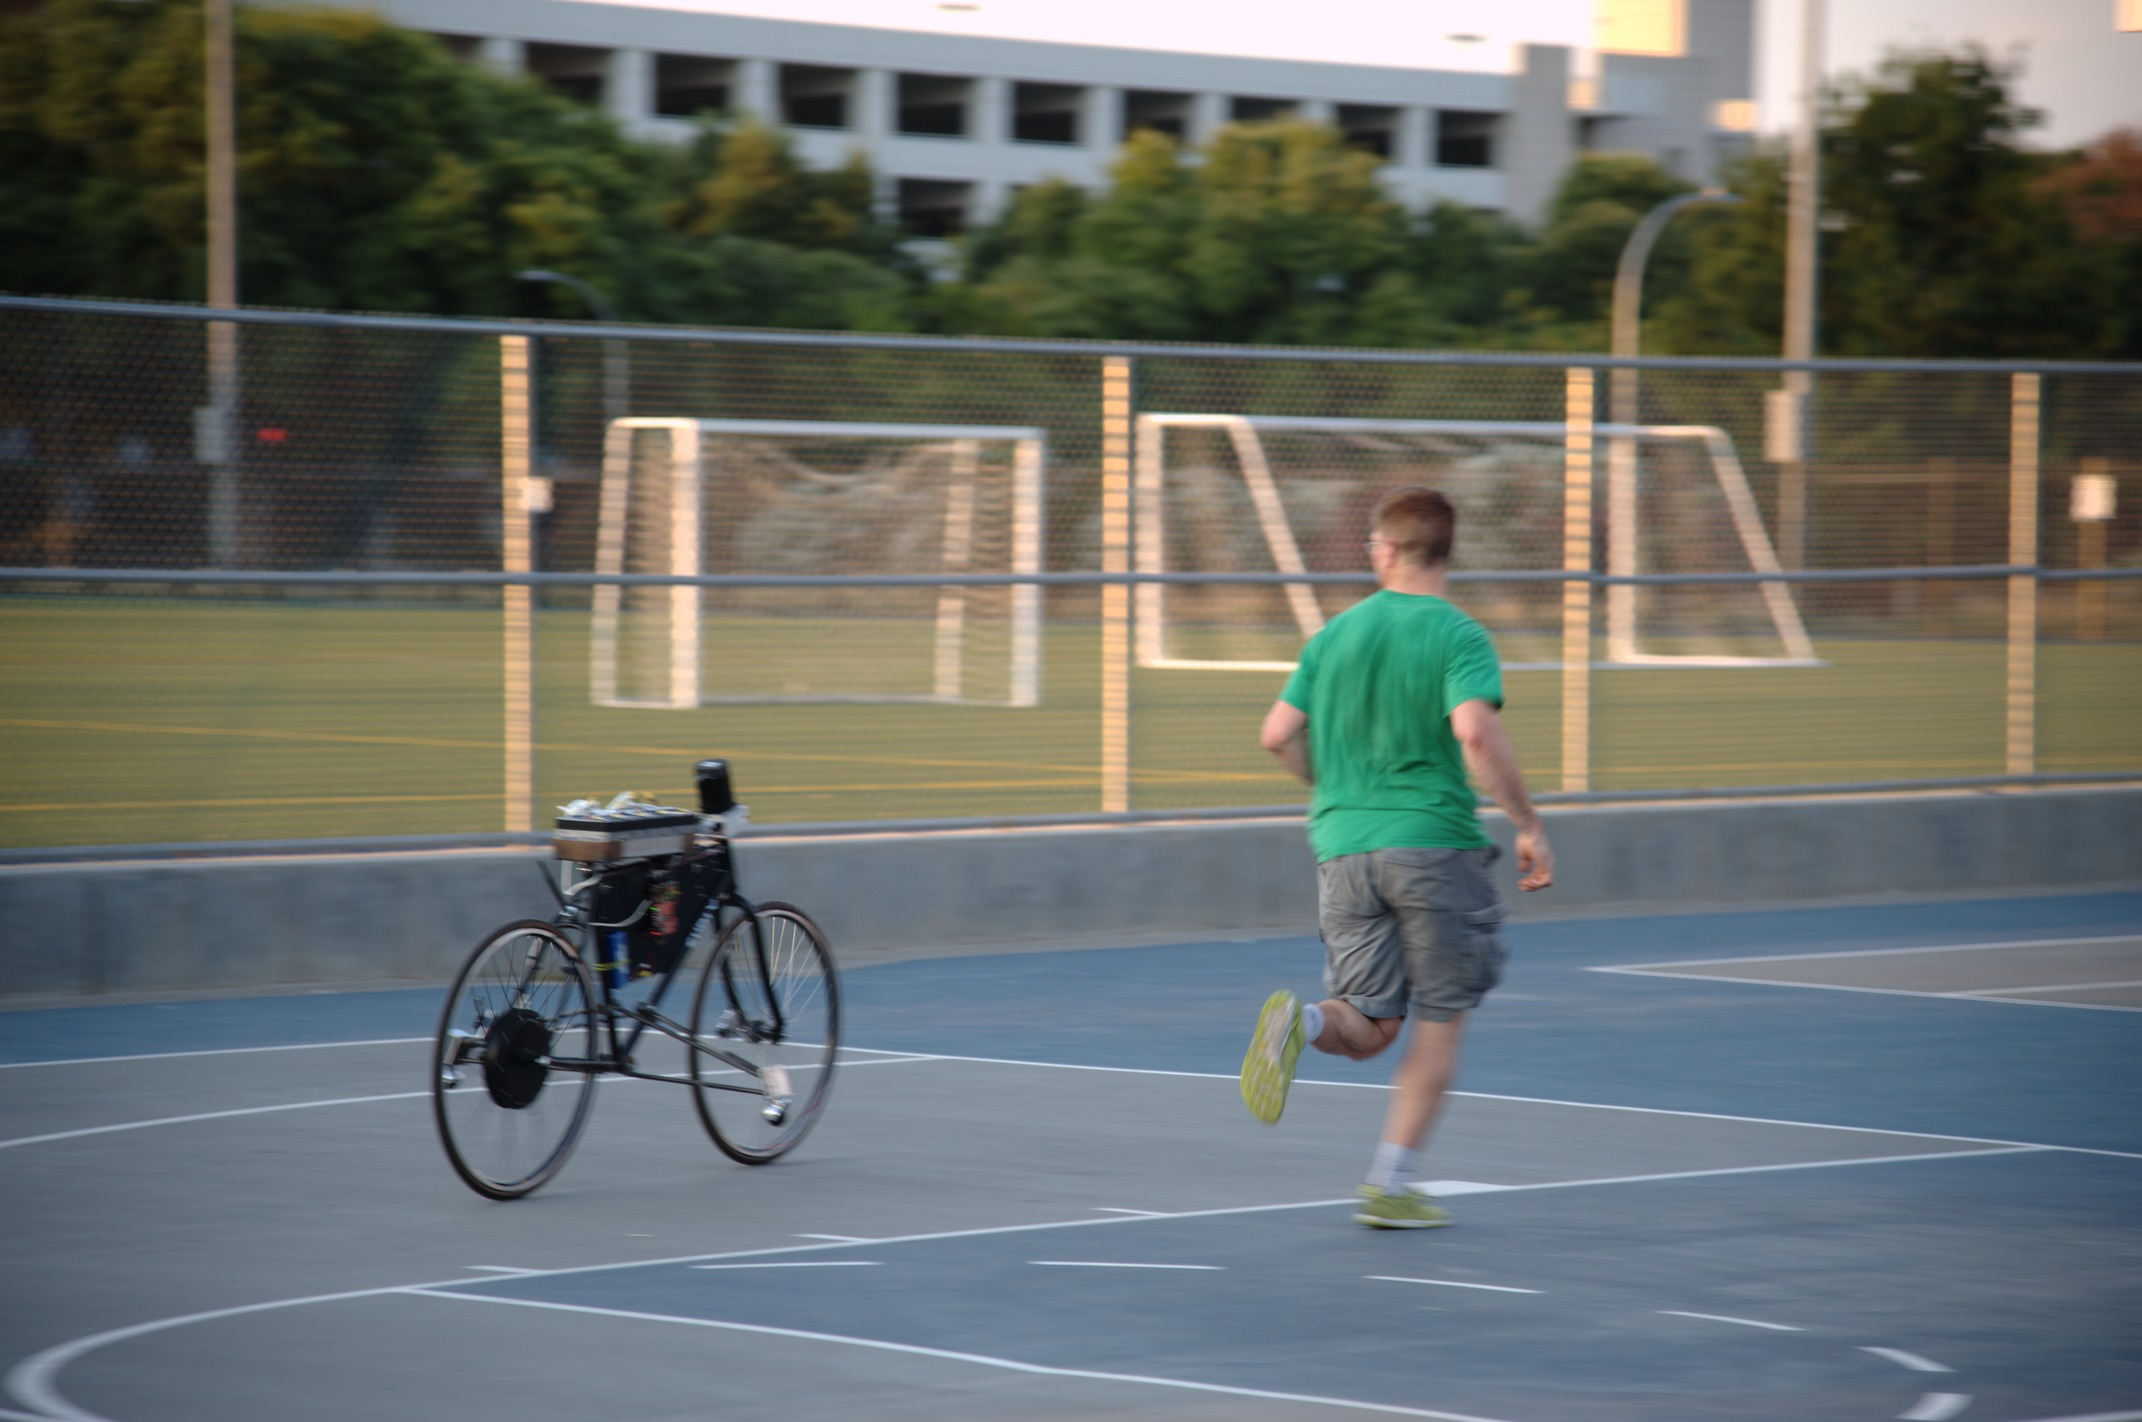
\includegraphics[width=\textwidth]{images/balancing.jpg}
  \caption{Taking the robot bicycle on a jog.}
  \label{balancing}
\end{figure}
\begin{figure}[!htbp]
  \pgfplotstableread{data/000_time_series_data_t20_t30-decimated.txt}\runzero
  \centering
  \begin{tikzpicture}
    % Lean estimate
    \begin{axis}[xlabel=Time (\si{\s}),
                 ylabel=Lean (\si{\radian}),name=plot1]
    \addplot[blue] table[x=time, y=lean_est]{\runzero}; \label{lean_est}
    \addlegendentry{$\hat{\phi}$}
    \end{axis}
    % Steer, steer estimate
    \begin{axis}[xlabel=Time (\si{\s}),
                 ylabel=Steer (\si{\radian}),name=plot2,at=(plot1.right of south east), anchor=left of south west]
    \addplot[red] table[x=time, y=steer]{\runzero}; \label{steer}
    \addlegendentry{$\delta$}
    \addplot[blue] table[x=time, y=steer_est]{\runzero}; \label{steer_est}
    \addlegendentry{$\hat{\delta}$}
    \end{axis}
    % Steer rate, steer rate estimate
    \begin{axis}[xlabel=Time (\si{\s}),
                 ylabel=Steer rate (\si{\radian\per\s}),name=plot4, at=(plot2.below south west), anchor=above north west]
    \addplot[red] table[x=time, y=steer_rate]{\runzero}; \label{steer_rate}
    \addlegendentry{$\dot{\delta}$}
    \addplot[blue] table[x=time, y=steer_rate_est]{\runzero}; \label{steer_rate_est}
    \addlegendentry{$\hat{\dot{\delta}}$}
    \end{axis}
    % Lean rate, lean rate estimate
    \begin{axis}[xlabel=Time (\si{\s}),
                 ylabel=Lean rate (\si{\radian\per\s}),name=plot3, at=(plot4.left of south west), anchor=right of south east]
    \addplot[red] table[x=time, y=gyro_x]{\runzero}; \label{lean_rate}
    \addlegendentry{$\dot{\phi}$}
    \addplot[blue] table[x=time, y=lean_rate_est]{\runzero}; \label{lean_rate_est}
    \addlegendentry{$\hat{\dot{\phi}}$}
    \end{axis}
  \end{tikzpicture}
  \caption{Estimator and measurement response during an experiment conducted at
    \SI{2.0}{\m\per\s}. No direct measurement of lean was available to compare
    with lean estimate.}
  \label{fig:run000}
\end{figure}

\section{Discussion} \label{sec:discussion}
The full-state estimator worked sufficiently well for the state feedback law to
stabilize the bicycle outside its stable speed range. However, it is clear from
\autoref{fig:run000} that the steer rate estimate $\hat{\dot{\delta}}$ was not
accurate. For example, at $t=\SI{25.0}{\s}$, the slope of the $\delta$ plot is
clearly negative, yet $\hat{\dot{\delta}}$ is positive at that time.

Besides the poor estimate of $\hat{\dot{\delta}}$, the other state estimates
seem reasonable.  The mean lean angle estimate $\mu_{\hat{\phi}} =
\SI{0.002}{\radian}$ over the time range presented is in agreement with our
observations that the bicycle turned slightly to the right over the course of
the run. The lean rate estimate $\hat{\dot{\phi}}$ closely follows the lean
rate measurement $\dot{\phi}$ but with slightly lower noise magnitudes.

\section{Conclusion} \label{sec:conclusion}
The state estimate, along with an LQR full-state feedback gain, was sufficient
to stabilize the robotic bicycle outside the stable speed range. More tuning is
needed to improve the estimate of steer rate. Additionally, a direct
measurement of the lean angle to which the lean angle estimate can be compared
would yield valuable information about the estimator performance. Lean angle is
the most heavily weighted state in the LQR gain so reducing lean angle
estimation error is especially desirable. Experimental testing with the
reduced-state estimator is needed to determine whether the potential increase
in bandwidth would be beneficial to balancing at speeds lower than
\SI{1.0}{\m\per\s}.

\section{Acknowledgements}
This paper is based on work supported by the National Science Foundation under
Grant No. 0928339.

\printbibliography

\end{document}

